\documentclass[journal]{IEEEtran}
\usepackage{cite}
\usepackage[pdftex]{graphicx}
\usepackage{tikz}
\usepackage[cmex10]{amsmath}
\usepackage{algorithmic}
\usepackage{array}
\usepackage[caption=false,font=normalsize,labelfont=sf,textfont=sf]{subfig}
\usepackage{url}
\usepackage{bbm}
\usepackage{listings}

\lstset{
    basicstyle=\ttfamily,
    frame=lrtb
}

\graphicspath{ {images/} }
\DeclareGraphicsExtensions{.pdf, .jpeg, .png}
\usetikzlibrary{ calc, trees, positioning, arrows, chains, shapes.geometric,
    decorations.pathreplacing, decorations.pathmorphing, shapes,
    matrix,shapes.symbols }

\tikzset{
    generic_node/.style={rectangle, rounded corners, minimum width=2.5cm, minimum height = 0.75cm, text centered, align=center, draw=black},
    center_text/.style={minimum width=2.5cm, text centered, align=center},
    arrow/.style={thick, ->, >=stealth},
    dashed_arrow/.style={->, >=stealth, dashed},
    line/.style={thick},
    rec/.style={rectangle, minimum height = 0.75cm, text centered,text depth=.25ex, align=center, draw=black},
    t_circ/.style={draw=black, circle, text centered, align=center},
    account_name/.style={minimum width = 1.5em, rectangle, text centered, align=center, draw=black},
    inv_account_name/.style={rectangle, text centered, align=center, minimum width = 1.5em},
}

% correct bad hyphenation here
\hyphenation{op-tical net-works semi-conduc-tor}

\makeatletter % Actually evenly spaced vdots
\DeclareRobustCommand{\rvdots}{%
  \vbox{
    \baselineskip4\p@\lineskiplimit\z@
    \kern-\p@
    \hbox{.}\hbox{.}\hbox{.}
  }}
\makeatother
\DeclareMathOperator*{\argmin}{arg\,min}
\DeclareMathOperator*{\argmax}{arg\,max}

\begin{document}
% paper title
% can use linebreaks \\ within to get better formatting as desired
% Do not put math or special symbols in the title.
\title{RaiBlocks: A Feeless Distributed Cryptocurrency Network}

% author names and IEEE memberships
% note positions of commas and nonbreaking spaces ( ~ ) LaTeX will not break
% a structure at a ~ so this keeps an author's name from being broken across
% two lines.
% use \thanks{} to gain access to the first footnote area
% a separate \thanks must be used for each paragraph as LaTeX2e's \thanks
% was not built to handle multiple paragraphs
\author{Colin LeMahieu\\clemahieu@gmail.com}% <-this % stops a space


% note the % following the last \IEEEmembership and also \thanks - 
% these prevent an unwanted space from occurring between the last author name
% and the end of the author line. i.e., if you had this:
% 
% \author{....lastname \thanks{...} \thanks{...} }
%                     ^------------^------------^----Do not want these spaces!
%
% a space would be appended to the last name and could cause every name on that
% line to be shifted left slightly. This is one of those ''LaTeX things''. For
% instance, ''\textbf{A} \textbf{B}'' will typeset as ''A B'' not ''AB''. To get
% ''AB'' then you have to do: ''\textbf{A}\textbf{B}''
% \thanks is no different in this regard, so shield the last } of each \thanks
% that ends a line with a % and do not let a space in before the next \thanks.
% Spaces after \IEEEmembership other than the last one are OK (and needed) as
% you are supposed to have spaces between the names. For what it is worth,
% this is a minor point as most people would not even notice if the said evil
% space somehow managed to creep in.


% make the title area
\maketitle

% As a general rule, do not put math, special symbols or citations
% in the abstract or keywords.
% \begin{abstract}
% While distributed cryptocurrencies have been around for several years, adoption has been low and initial adopter markets have failed to materialize.

% Compared to a centralized system, the transaction performance of these systems are significantly worse, relegating them to niche markets that primarily capitalize on the benefits of decentralization at the cost of speed or expense. RaiBlocks is designed to solve performance and cost problems while retaining properties of currency and decentralization.

% Our approach uses two high level observations: run-time agreements are slower than design time agreements and complexity only increases agreement time rather than lowering it.
% \end{abstract}

\begin{abstract}
    Recently, high demand and limited scalability have increased the average transaction times and fees in popular cryptocurrencies, yielding an unsatisfactory experience. Here we introduce RaiBlocks, a cryptocurrency with a novel block-lattice architecture where each account has its own blockchain, delivering near instantaneous transaction speed and unlimited scalability. Each user has their own blockchain, allowing them to update it asynchronously to the rest of the network, resulting in fast transactions with minimal overhead. Transactions keep track of account balances rather than transaction amounts, allowing aggressive database pruning without compromising security. To date, the RaiBlocks network has processed 4.2 million transactions with an unpruned ledger size of only 1.7GB. RaiBlock's feeless, split-second transactions make it the premier cryptocurrency for consumer transactions.
\end{abstract}

% Background (1 sentence)
% Problem statement (1 sentence)
% Solution (however many sentences)
% Observation (key results, performance, whatever; few sentence)
% Conclusion (few sentences)
% Most important (last sentence)

% Note that keywords are not normally used for peerreview papers.
\begin{IEEEkeywords}
cryptocurrency, blockchain, raiblocks, distributed ledger, digital, transactions
\end{IEEEkeywords}


% For peer review papers, you can put extra information on the cover
% page as needed:
% \ifCLASSOPTIONpeerreview
% \begin{center} \bfseries EDICS Category: 3-BBND \end{center}
% \fi
%
% For peerreview papers, this IEEEtran command inserts a page break and
% creates the second title. It will be ignored for other modes.
\IEEEpeerreviewmaketitle



\section{Introduction}
% Status: First Draft; Ready for Review
\IEEEPARstart{S}{ince} the implementation of Bitcoin in 2009, there has been a growing shift away from traditional, government-backed currencies and financial systems towards modern payments systems based on cryptography, which offer the ability to store and transfer funds in a trustless and secure manner \cite{Nakamoto_bitcoin:a}. In order to function effectively, a currency must be easily transferable, non-reversible, and have limited or no fees. The increased transaction times, large fees, and questionable network scalability have raised questions about the practicality of Bitcoin as an everyday currency.

In this paper, we introduce Nano, a low-latency cryptocurrency built on an innovative block-lattice data structure offering unlimited scalability and no transaction fees. Nano by design is a simple protocol with the sole purpose of being a high-performance cryptocurrency. The Nano protocol can run on low-power hardware, allowing it to be a practical, decentralized cryptocurrency for everyday use.

Cryptocurrency statistics reported in this paper are accurate as of publication date.

\section{Background}
% Status: First Draft; Ready for Review
% Even though this figure doesn't belong in this section, it's placed here for better placement in the rendered paper.
\begin{figure*}[!ht]
  \centering
  \subfloat[a][When no conflict is detected, no further overhead is required.]{
    \centering
    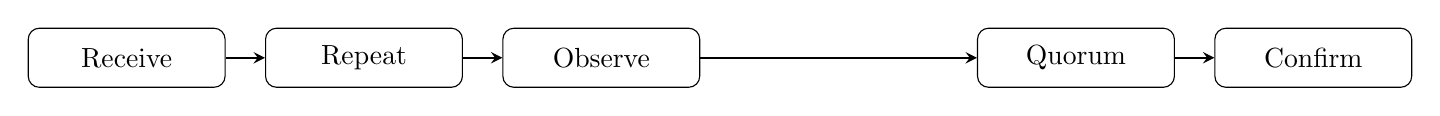
\begin{tikzpicture}[node distance=0.5cm]
      %%%%%%%%%%%%%%%
      % No Conflict %
      %%%%%%%%%%%%%%%
      \node (receive) [generic_node]
          {Receive};
      \node (repeat) [generic_node, right = of receive]
          {Repeat};
      \node (observe) [generic_node, right = of repeat]
          {Observe};
      \node (fake) [center_text, right = of observe]{};
      \node (quorum) [generic_node, right = of fake] 
          {Quorum};
      \node (confirm) [generic_node, right = of quorum]
          {Confirm};
      
      \draw [arrow] (receive) -- (repeat);
      \draw [arrow] (repeat) -- (observe);
      \draw [arrow] (observe) -- (quorum);
      \draw [arrow] (quorum) -- (confirm);
      
    \end{tikzpicture}
  }
  \newline
  \subfloat[b][In the event of a conflicting transaction, nodes vote for the valid transaction.]{
    \centering
    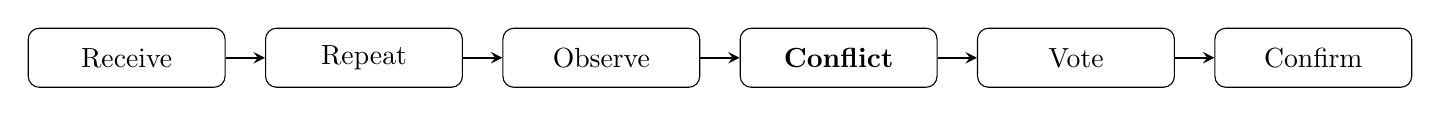
\begin{tikzpicture}[node distance=0.5cm]
      %%%%%%%%%%%%
      % Conflict %
      %%%%%%%%%%%%
      \node (receive) [generic_node]
          {Receive};
      \node (repeat) [generic_node, right = of receive]
          {Repeat};
      \node (observe) [generic_node, right = of repeat]
          {Observe};
      \node (conflict) [generic_node, right = of observe]
          {\textbf{Conflict}};
      \node (vote) [generic_node, right = of conflict] 
          {Vote};
      \node (confirm) [generic_node, right = of vote]
          {Confirm};
      
      \draw [arrow] (receive) -- (repeat);
      \draw [arrow] (repeat) -- (observe);
      \draw [arrow] (observe) -- (conflict);
      \draw [arrow] (conflict) -- (vote);
      \draw [arrow] (vote) -- (confirm);
      
    \end{tikzpicture}
  }
  \caption{Nano requires no additional overhead for typical transactions. In the event of conflicting transactions, nodes must vote for the transaction to keep}
  \label{fig:transaction_flow}
\end{figure*}

In 2008, an anonymous individual under the pseudonym Satoshi Nakamoto published a whitepaper outlining the world's first decentralized cryptocurrency, Bitcoin \cite{Nakamoto_bitcoin:a}. A key innovation brought about by Bitcoin was the blockchain, a public, immutable and decentralized data-structure which is used as a ledger for the currency's transactions. Unfortunately, as Bitcoin matured, several issues in the protocol made Bitcoin prohibitive for many applications:
\begin{enumerate}
  \item Poor scalability: Each block in the blockchain can store a limited amount of data, which means the system can only process so many transactions per second, making spots in a block a commodity. Currently the median transaction fee is \$10.38 \cite{Bitcoin_med_fee}.
  \item High latency: The average confirmation time is 164 minutes \cite{Bitcoin_avg_confirmation_time}.
  \item Power inefficient: The Bitcoin network consumes an estimated 27.28TWh per year, using on average 260KWh per transaction \cite{Bitcoin_energy_index}.
\end{enumerate}

Bitcoin, and other cryptocurrencies, function by achieving consensus on their global ledgers in order to verify legitimate transactions while resisting malicious actors. Bitcoin achieves consensus via an economic measure called Proof of Work (PoW). In a PoW system participants compete to compute a number, called a \textit{nonce}, such that the hash of the entire block is in a target range. This valid range is inversely proportional to the cumulative computation power of the entire Bitcoin network in order to maintain a consistent average time taken to find a valid nonce. The finder of a valid nonce is then allowed to add the block to the blockchain; therefore, those who exhaust more computational resources to compute a nonce play a greater role in the state of the blockchain. PoW provides resistance against a Sybil attack, where an entity behaves as multiple entities to gain additional power in a decentralized system, and also greatly reduces race conditions that inherently exist while accessing a global data-structure.

An alternative consensus protocol, Proof of Stake (PoS), was first introduced by Peercoin in 2012 \cite{King_peercoin}. In a PoS system, participants vote with a weight equivalent to the amount of wealth they possess in a given cryptocurrency. With this arrangement, those who have a greater financial investment are given more power and are inherently incentivized to maintain the honesty of the system or risk losing their investment. PoS does away with the wasteful computation power competition, only requiring light-weight software running on low power hardware.

The original Nano (RaiBlocks) paper and first beta implementation were published in December, 2014, making it one of the first Directed Acyclic Graph (DAG) based cryptocurrencies \cite{Colin_original_Raiblocks}. Soon after, other DAG cryptocurrencies began to develop, most notably DagCoin/Byteball and IOTA \cite{Ribero_dagcoin:a, Popov_tangle:a}. These DAG-based cryptocurrencies broke the blockchain mold, improving system performance and security. Byteball achieves consensus by relying on a ``main-chain'' comprised of honest, reputable and user-trusted ``witnesses'', while IOTA achieves consensus via the cumulative PoW of stacked transactions. Nano achieves consensus via a balance-weighted vote on conflicting transactions. This consensus system provides quicker, more deterministic transactions while still maintaining a strong, decentralized system. Nano continues this development and has positioned itself as one of the highest performing cryptocurrencies.


\section{RaiBlocks Components}
% Status: First Draft; Ready for Review
Before describing the overall Nano architecture, we define the individual components that make up the system.

\subsection{Account}
An account is the public-key portion of a digital signature key-pair. The public-key, also referred to as the address, is shared with other network participants while the private-key is kept secret. A digitally signed packet of data ensures that the contents were approved by the private-key holder. One user may control many accounts, but only one public address may exist per account.

\begin{figure}[!b]
      \centering
      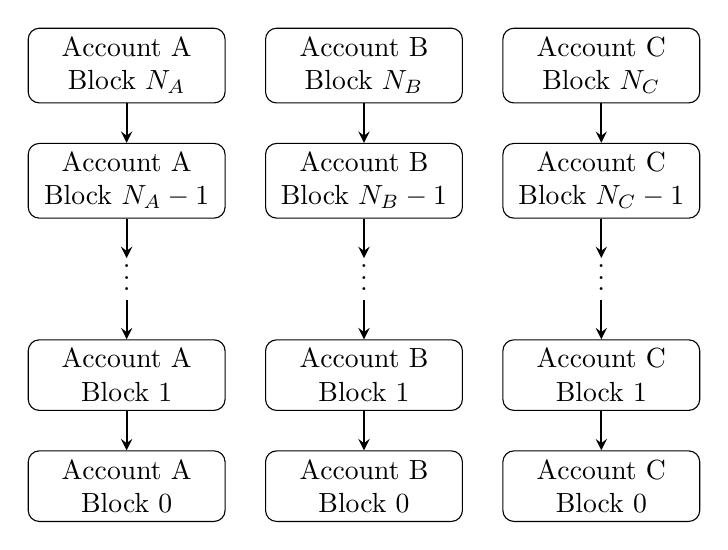
\begin{tikzpicture}[node distance=0.5cm]
            %%%%%%%%%%%%%
            % ACCOUNT A %
            %%%%%%%%%%%%%
            \node (account_A_head) [generic_node]
                    {Account A \\ Block $N_A$};
            \node (account_A_prev) [generic_node, below = of account_A_head]
                    {Account A \\   Block $N_A-1$};
            \node (account_A_ellipsis) [center_text, below=of account_A_prev]
                    {$\rvdots$};
            \node (account_A_1) [generic_node, below = of account_A_ellipsis] 
                    {Account A \\   Block $1$};
            \node (account_A_0) [generic_node, below = of account_A_1]
                    {Account A \\   Block $0$};
            
            \draw [arrow] (account_A_head) -- (account_A_prev);
            \draw [arrow] (account_A_prev) -- (account_A_ellipsis);
            \draw [arrow] (account_A_ellipsis) -- (account_A_1);
            \draw [arrow] (account_A_1) -- (account_A_0);
            
            %%%%%%%%%%%%%
            % ACCOUNT B %
            %%%%%%%%%%%%%
            \node (account_B_head) [generic_node, right = of account_A_head]
                    {Account B \\ Block $N_B$};
            \node (account_B_prev) [generic_node, below = of account_B_head]
                    {Account B \\   Block $N_B-1$};
            \node (account_B_ellipsis) [center_text, below=of account_B_prev]
                    {$\rvdots$};
            \node (account_B_1) [generic_node, below = of account_B_ellipsis] 
                    {Account B \\   Block $1$};
            \node (account_B_0) [generic_node, below = of account_B_1]
                    {Account B \\   Block $0$};
            
            \draw [arrow] (account_B_head) -- (account_B_prev);
            \draw [arrow] (account_B_prev) -- (account_B_ellipsis);
            \draw [arrow] (account_B_ellipsis) -- (account_B_1);
            \draw [arrow] (account_B_1) -- (account_B_0);
            
            %%%%%%%%%%%%%
            % ACCOUNT C %
            %%%%%%%%%%%%%
            \node (account_C_head) [generic_node, right = of account_B_head]
                    {Account C \\ Block $N_C$};
            \node (account_C_prev) [generic_node, below = of account_C_head]
                    {Account C \\   Block $N_C-1$};
            \node (account_C_ellipsis) [center_text, below=of account_C_prev]
                    {$\rvdots$};
            \node (account_C_1) [generic_node, below = of account_C_ellipsis] 
                    {Account C \\   Block $1$};
            \node (account_C_0) [generic_node, below = of account_C_1]
                    {Account C \\   Block $0$};
            
            \draw [arrow] (account_C_head) -- (account_C_prev);
            \draw [arrow] (account_C_prev) -- (account_C_ellipsis);
            \draw [arrow] (account_C_ellipsis) -- (account_C_1);
            \draw [arrow] (account_C_1) -- (account_C_0);
      \end{tikzpicture}
      \caption{Each account has its own blockchain containing the account's balance history. Block 0 must be an open transaction (Section~\ref{sec:open})}
      \label{fig:account_chain}
\end{figure}

\subsection{Block/Transaction}
The term ``block'' and ``transaction'' are often used interchangeably, where a block contains a single transaction. Transaction specifically refers to the action while block refers to the digital encoding of the transaction. Transactions are signed by the private-key belonging to the account on which the transaction is performed.

\subsection{Ledger}
The ledger is the global set of accounts where each account has its own transaction chain (Figure~\ref{fig:account_chain}). This is a key design component that falls under the category of replacing a run-time agreement with a design-time agreement; everyone agrees via signature checking that only an account owner can modify their own chain. This converts a seemingly shared data-structure, a distributed ledger, in to a set of non-shared ones.

\subsection{Node}
A \textit{node} is a piece of software running on a computer that conforms to the Nano protocol and participates in the Nano network. The software manages the ledger and any accounts the node may control, if any. A node may either store the entire ledger or a pruned history containing only the last few block of each account's blockchain. When setting up a new node it is recommended to verify the entire history and prune locally.

\section{System Overview}
% Status: First Draft; Ready for Review
Unlike blockchains used in many other cryptocurrencies, Nano uses a \textit{block-lattice} structure. Each account has its own blockchain (account-chain) equivalent to the account's transaction/balance history (Figure \ref{fig:account_chain}). Each account-chain can only be updated by the account's owner; this allows each account-chain to be updated immediately and asynchronously to the rest of the block-lattice, resulting in quick transactions. Nano's protocol is extremely light-weight; each transaction fits within the required minimum UDP packet size for being transmitted over the internet. Hardware requirements for nodes are also minimal, since nodes only have to record and rebroadcast blocks for most transactions (Figure \ref{fig:transaction_flow}).

The system is initiated with a \textit{genesis account} containing the \textit{genesis balance}. The genesis balance is a fixed quantity and can never be increased. The genesis balance is divided and sent to other accounts via send transactions registered on the genesis account-chain. The sum of the balances of all accounts will never exceed the initial genesis balance which gives the system an upper bound on quantity and no ability to increase it.

This section will walk through how different types of transactions are constructed and propagated throughout the network.

\begin{figure}[!ht]
   \centering
   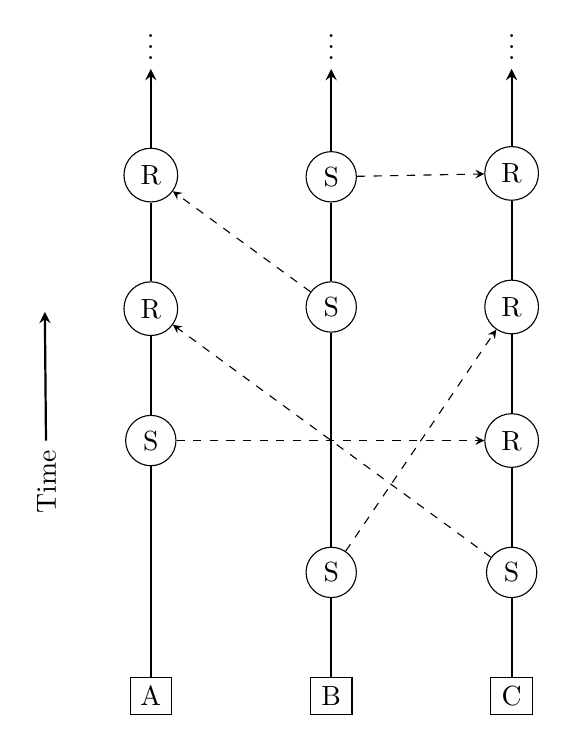
\begin{tikzpicture}[node distance=1cm]
      \node (a) [account_name]{A};
      \node (b) [account_name, right = of a, xshift=0.75cm]{B};
      \node (c) [account_name, right = of b, xshift=0.75cm]{C};
            
      \node (c_1) [t_circ, above = of c, yshift=0cm]{S};
      \node (c_2) [t_circ, above = of c_1, yshift=0cm]{R};
      \node (c_3) [t_circ, above = of c_2, yshift=0cm]{R};
      \node (c_4) [t_circ, above = of c_3, yshift=0cm]{R};
      
      \node (a_1) at (c_2-| a)[t_circ]{S};
      \node (a_2) [t_circ, above = of a_1, yshift=0cm]{R};
      \node (a_3) [t_circ, above = of a_2, yshift=0]{R};
            
      \node (b_1) at (c_1 -| b) [t_circ]{S};
      \node (b_2) at (c_3 -| b) [t_circ]{S};
      \node (b_3) [t_circ, above = of b_2]{S};
            
      \node (a_ellipsis) [inv_account_name, above=of a_3]{$\rvdots$};
      \node (b_ellipsis) at (a_ellipsis -| b) [inv_account_name]{$\rvdots$};
      \node (c_ellipsis) at (a_ellipsis -| c) [inv_account_name]{$\rvdots$};

      \draw [line] (a) -- (a_1);
      \draw [line] (a_1) -- (a_2);
      \draw [line] (a_2) -- (a_3);
      \draw [arrow] (a_3) -- (a_ellipsis);
      
      \draw [line] (b) -- (b_1);
      \draw [line] (b_1) -- (b_2);
      \draw [line] (b_2) -- (b_3);
      \draw [arrow] (b_3) -- (b_ellipsis);
      
      \draw [line] (c) -- (c_1);
      \draw [line] (c_1) -- (c_2);
      \draw [line] (c_2) -- (c_3);
      \draw [line] (c_3) -- (c_4);
      \draw [arrow] (c_4) -- (c_ellipsis);
      
      \draw [dashed_arrow] (c_1) -- (a_2);
      \draw [dashed_arrow] (b_1) -- (c_3);
      \draw [dashed_arrow] (b_3) -- (c_4);
      \draw [dashed_arrow] (a_1) -- (c_2);
      \draw [dashed_arrow] (b_2) -- (a_3);
      
      \node (time)[inv_account_name, rotate=90, left=of a_1]{Time};
      \node (e_time)[inv_account_name, left=of a_2, rotate=90, xshift=0.5cm]{};
      
      \draw [arrow] (time) -- (e_time);
   \end{tikzpicture}
   \caption{Visualization of the block-lattice. Every transfer of funds requires a send block (S) and a receive block (R), each signed by their account-chain's owner (A,B,C)}
   \label{fig:cross_account_chain}
\end{figure}

\subsection{Transactions} \label{sec:transactions}
Transferring funds from one account to another requires two transactions: a \textit{send} deducting the amount from the sender's balance and a \textit{receive} adding the amount to the receiving account's balance (Figure~\ref{fig:cross_account_chain}).

Transferring amounts as separate transactions in the sender's and receiver's accounts serves a few important purposes:
\begin{enumerate}
   \item Sequencing incoming transfers that are inherently asynchronous.
   \item Keeping transactions small to fit in UDP packets.
   \item Facilitating ledger pruning by minimizing the data footprint.
   \item Isolating settled transactions from unsettled ones.
\end{enumerate}

More than one account transferring to the same destination account is an asynchronous operation; network latency and the sending accounts not necessarily being in communication with each other means there is no universally agreeable way to know which transaction happened first. Since addition is associative, the order the inputs are sequenced does not matter, and hence we simply need a global agreement. This is a key design component that converts a run-time agreement in to a design-time agreement. The receiving account has control over deciding which transfer arrived first and is expressed by the signed order of the incoming blocks.

If an account wants to make a large transfer that was received as a set of many small transfers, we want to represent this in a way that fits within a UDP packet. When a receiving account sequences input transfers, it keeps a running total of its account balance so that at any time it has the ability to transfer any amount with a fixed size transaction. This differs from the input/output transaction model used by Bitcoin and other cryptocurrencies.

Some nodes are uninterested in expending resources to store an account's full transaction history; they are only interested in each account's current balance. When an account makes a transaction, it encodes its accumulated balance and these nodes only need to keep track of the latest block, which allows them to discard historical data while maintaining correctness.

Even with a focus on design-time agreements, there is a delay window when validating transactions due to identifying and handling bad actors in the network. Since agreements in Nano are reached quickly, on the order of milliseconds to seconds, we can present the user with two familiar categories of incoming transactions: settled and unsettled. Settled transactions are transactions where an account has generated receive blocks. Unsettled transactions have not yet been incorporated in to the receiver's cumulative balance. This is a replacement for the more complex and unfamiliar confirmations metric in other cryptocurrencies.

\subsection{Creating an Account}\label{sec:open}
To create an account, you need to issue an \textit{open} transaction (Figure~\ref{code:open}). An open transaction is always the first transaction of every account-chain and can be created upon the first receipt of funds. The \textit{account} field stores the public-key (address) derived from the private-key that is used for signing. The \textit{source} field contains the hash of the transaction that sent the funds. On account creation, a representative must be chosen to vote on your behalf; this can be changed later (Section~\ref{sec:change}). The account can declare itself as its own representative.

\begin{figure}[!ht]
\begin{lstlisting}
open {
   account: DC04354B1...AE8FA2661B2,
   source: DC1E2B3F7C...182A0E26B4A,
   representative: xrb_1anr...posrs,
   work: 0000000000000000,
   type: open,
   signature: 83B0...006433265C7B204
}
\end{lstlisting}
\caption{Anatomy of an open transaction}
\label{code:open}
\end{figure}

\subsection{Account Balance}\label{sec:account_balance}
The account balance is recorded within the ledger itself. Rather than recording the amount of a transaction, verification (Section~\ref{sec:transaction_verification}) requires checking the difference between the balance at the send block and the balance of the preceding block. The receiving account may then increment the previous balance as measured into the final balance given in the new receive block. This is done to improve processing speed when downloading high volumes of blocks. When requesting account history, amounts are already given.

\subsection{Sending From an Account} \label{sec:send}
To send from an address, the address must already have an existing open block, and therefore a balance (Figure~\ref{code:send}). The \textit{previous} field contains the hash of the previous block in the account-chain. The \textit{destination} field contains the account for funds to be sent to. A send block is immutable once confirmed. Once broadcasted to the network, funds are immediately deducted from the balance of the sender’s account and wait as \textit{pending} until the receiving party signs a block to accept these funds. Pending funds should not be considered awaiting confirmation, as they are as good as spent from the sender’s account and the sender cannot revoke the transaction.

\begin{figure}[!ht]
\begin{lstlisting}
send {
   previous: 1967EA355...F2F3E5BF801,
   balance: 010a8044a0...1d49289d88c,
   destination: xrb_3w...m37goeuufdp,
   work: 0000000000000000,
   type: send,
   signature: 83B0...006433265C7B204
}
\end{lstlisting}
\caption{Anatomy of a send transaction}
\label{code:send}
\end{figure}

\subsection{Receiving a Transaction}\label{sec:receive}
To complete a transaction, the recipient of sent funds must create a receive block on their own account-chain (Figure~\ref{code:receive}). The source field references the hash of the associated send transaction. Once this block is created and broadcasted, the account’s balance is updated and the funds have officially moved into their account.

\begin{figure}[!ht]
\begin{lstlisting}
receive {
   previous: DC04354B1...AE8FA2661B2,
   source: DC1E2B3F7C6...182A0E26B4A,
   work: 0000000000000000,
   type: receive,
   signature: 83B0...006433265C7B204
}
\end{lstlisting}
\caption{Anatomy of a receive transaction}
\label{code:receive}
\end{figure}

\subsection{Assigning a Representative}\label{sec:change}
Account holders having the ability to choose a representative to vote on their behalf is a powerful decentralization tool that has no strong analog in Proof of Work or Proof of Stake protocols. In conventional PoS systems, the account owner's node must be running to participate in voting. Continuously running a node is impractical for many users; giving a representative the power to vote on an account's behalf relaxes this requirement. Account holders have the ability to reassign consensus to any account at any time. A \textit{change} transaction changes the representative of an account by subtracting the vote weight from the old representative and adding the weight to the new representative (Figure~\ref{code:change}). No funds are moved in this transaction, and the representative does not have spending power of the account's funds.

\begin{figure}[!ht]
\begin{lstlisting}
change {
   previous: DC04354B1...AE8FA2661B2,
   representative: xrb_1anrz...posrs,
   work: 0000000000000000,
   type: change,
   signature: 83B0...006433265C7B204
}
\end{lstlisting}
\caption{Anatomy of a change transaction}
\label{code:change}
\end{figure}

\subsection{Forks and Voting} \label{sec:forks}
A fork occurs when $j$ signed blocks $b_1, b_2, \dots, b_j$ claim the same block as their predecessor (Figure \ref{fig:fork}). These blocks cause a conflicting view on the status of an account and must be resolved. Only the account's owner has the ability to sign blocks into their account-chain, so a fork must be the result of poor programming or malicious intent (double-spend) by the account's owner.

\begin{figure}[!ht]
   \centering
   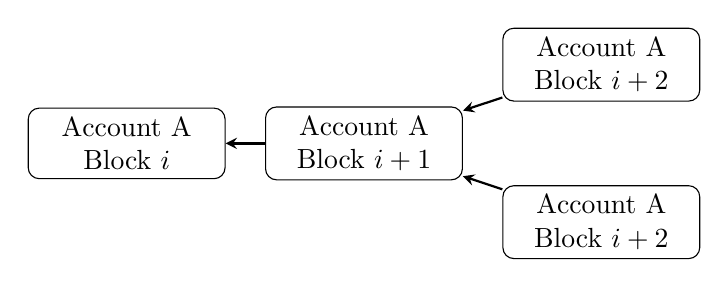
\begin{tikzpicture}[node distance=0.5cm]
      %%%%%%%%%%%%%
      % ACCOUNT A %
      %%%%%%%%%%%%%
      \node (account_A_0) [generic_node]
            {Account A \\ Block $i$};
      \node (account_A_1) [generic_node, right = of account_A_0]
            {Account A \\ Block $i+1$};
      \node (account_A_2a) [generic_node, right = of account_A_1, yshift=1cm] 
            {Account A \\ Block $i+2$};
      \node (account_A_2b) [generic_node, right = of account_A_1, yshift=-1cm]
            {Account A \\ Block $i+2$};
      
      \draw [arrow] (account_A_1) -- (account_A_0);
      \draw [arrow] (account_A_2a) -- (account_A_1);
      \draw [arrow] (account_A_2b) -- (account_A_1);
   \end{tikzpicture}
   \caption{A fork occurs when two (or more) signed blocks reference the same previous block. Older blocks are on the left; newer blocks are on the right}
   \label{fig:fork}
\end{figure}

Upon detection, a representative will create a vote referencing the block $\hat{b}_i$ in its ledger and broadcast it to the network. The weight of a node's vote, $w_i$, is the sum of the balances of all accounts that have named it as its representative. The node will observe incoming votes from the other $M$ online representatives and keep a cumulative tally for 4 voting periods, 1 minute total, and confirm the winning block (Equation \ref{eq:weighted_vote}).

\begin{align}
   v(b_j) &= \sum_{i=1}^M w_i\mathbbm{1}_{\hat{b}_i=b_j} \label{eq:weighted_vote} \\
   b^* &= \argmax_{b_j} v(b_j) \label{eq:most_votes}
\end{align}

The most popular block $b^*$ will have the majority of the votes and will be retained in the node's ledger (Equation~\ref{eq:most_votes}). The block(s) that lose the vote are discarded. If a representative replaces a block in its ledger, it will create a new vote with a higher sequence number and broadcast the new vote to the network. This is the \textbf{only} scenario where representatives vote.

In some circumstances, brief network connectivity issues may cause a broadcasted block to not be accepted by all peers. Any subsequent block on this account will be ignored as invalid by peers that did not see the initial broadcast. A rebroadcast of this block will be accepted by the remaining peers and subsequent blocks will be retrieved automatically. Even when a fork or missing block occurs, only the accounts referenced in the transaction are affected; the rest of the network proceeds with processing transactions for all other accounts.

\subsection{Proof of Work} \label{sec:pow}
All four transaction types have a work field that must be correctly populated. The work field allows the transaction creator to compute a nonce such that the hash of the nonce concatenated with the previous field in receive/send/change transactions or the account field in an open transaction is below a certain threshold value. Unlike Bitcoin, the PoW in Nano is simply used as an anti-spam tool, similar to Hashcash, and can be computed on the order of seconds \cite{Back_hashcash}. Once a transaction is sent, the PoW for the subsequent block can be precomputed since the previous block field is known; this will make transactions appear instantaneous to an end-user so long as the time between transactions is greater than the time required to compute the PoW.

\subsection{Transaction Verification} \label{sec:transaction_verification}
For a block to be considered valid, it must have the following attributes:
\begin{enumerate}
   \item The block must not already be in the ledger (duplicate transaction).
   \item Must be signed by the account's owner.
   \item The previous block is the head block of the account-chain. If it exists but is not the head, it is a fork.
   \item The account must have an open block.
   \item The computed hash meets the PoW threshold requirement.
\end{enumerate}
If it is a receive block, check if the source block hash is pending, meaning it has not already been redeemed. If it is a send block, the balance must be less than the previous balance.

\section{Attack Vectors}
% Status: First Draft; NOT Ready for Review
RaiBlocks, like all decentralized cryptocurrencies, may be attacked by malicious parties for attempted financial gain or system demise. In this section we outline a few possible attack scenarios, the consequences of such an attack, and how RaiBlock's protocol takes preventative measures.

\subsection{Block Gap Synchronization}
In Section~\ref{sec:forks}, we discussed the scenario where a block may not be properly broadcasted, causing the network to ignore subsequent blocks. If a node observes a block that does not have the referenced previous block, it has two options:
\begin{enumerate}
  \item Ignore the block as it might be a malicious garbage block.
  \item Request a resync with another node.
\end{enumerate}
In the case of a resync, a TCP connection must be formed with a bootstrapping node to facilitate the increased amount of traffic a resync requires. However, if the block was actually a bad block, then the resync was unnecessary and needlessly increased traffic on the network. This is a Network Amplification Attack and results in a denial-of-service.

To avoid unnecessary resyncing, nodes will wait until a certain threshold of votes have been observed for a potentially malicious block before initiating a connection to a bootstrap node to synchronize. If a block doesn't receive enough votes it can be assumed to be junk data.

\subsection{Transaction Flooding}\label{sec:transaction_flooding}
A malicious entity could send many unnecessary but valid transactions between accounts under its control in an attempt to saturate the network. With no transaction fees they are able to continue this attack indefinitely. However, the PoW required for each transaction limits the transaction rate the malicious entity could generate without significantly investing in computational resources. Even under such an attack in an attempt to inflate the ledger, nodes that are not full historical nodes are able to prune old transactions from their chain; this clamps the storage usage from this type of attack for almost all users.

\subsection{Sybil Attack}
An entity could create hundreds of RaiBlocks nodes on a single machine; however, since the voting system is weighted based on account balance, adding extra nodes in to the network will not gain an attacker extra votes. Therefore there is no advantage to be gained via a Sybil attack.

\subsection{Penny-Spend Attack}
A penny-spend attack is where an attacker spends infinitesimal quantities to a large number of accounts in order to waste the storage resources of nodes. Block publishing is rate-limited by the PoW, so this limits the creation of accounts and transactions to a certain extent. Nodes that are not full historical nodes can prune accounts below a statistical metric where the account is most likely not a valid account. Finally, RaiBlocks is tuned to use minimal permanent storage space, so space required to store one additional account is proportional to the size of an $\text{open block} + \text{indexing} = 96\text{B} + 32\text{B} = 128\text{B}$. This equates to 1GB being able to store 8 million penny-spend account. If nodes wanted to prune more aggressively, they can calculate a distribution based on access frequency and delegate infrequently used accounts to slower storage.

\subsection{Precomputed PoW Attack}
Since the owner of an account will be the only entity adding blocks to the account-chain, sequential blocks can be computed, along with their PoW, before being broadcasted to the network. Here the attacker generates a myriad of sequential blocks, each of minimal value, over an extended period of time. At a certain point, the attacker performs a Denial of Service (DoS) by flooding the network with lots of valid transactions, which other nodes will process and echo as quickly as possible. This is an advanced version of the transaction flooding described in Section~\ref{sec:transaction_flooding}. Such an attack would only work briefly, but could be used in conjunction with other attacks, such as a \textgreater 50\% Attack (Section~\ref{sec:attack_50}) to increase effectiveness. Transaction rate-limiting and other techniques are currently being investigated to mitigate attacks.

\subsection{\textgreater 50\% Attack} \label{sec:attack_50}
The metric of consensus for RaiBlocks is a balance weighted voting system. If an attacker is able to gain over 50\% of the voting strength, they can cause the network to oscillate consensus rendering the system broken. An attacker is able to lower the amount of balance they must forfeit by preventing good nodes from voting through a network DoS. RaiBlocks takes the following measures to prevent such an attack:
\begin{enumerate}
  \item The primary defense against this type of attack is voting-weight being tied to investment in the system. An account holder is inherently incentivized to maintain the honesty of the system to protect their investment. Attempting to flip the ledger would be destructive to the system as a whole which would destroy their investment.
  
  \item The cost of this attack is proportional to the market capitalization of RaiBlocks. In PoW systems, technology can be invented that gives disproportionate control compared to monetary investment and if the attack is successful, this technology could be repurposed after the attack is complete. With RaiBlocks the cost of attacking the system scales with the system itself and if an attack were to be successful the investment in the attack cannot be recovered.

  
  \item In order to maintain the maximum quorum of voters, the next line of defense is representative voting. Account holders who are unable to reliably participate in voting for connectivity reasons can name a representative who can vote with the weight of their balance. Maximizing the number and diversity of representatives increases network resiliency.
  
  \item Forks in RaiBlocks are never accidental, so nodes can make policy decisions on how to interact with forked blocks. The only time non-attacker accounts are vulnerable to block forks is if they receive a balance from an attacking account. Accounts wanting to be secure from block forks can wait a little or a lot longer before receiving from an account who generated forks or opt to never receive at all. Receivers could also generate separate accounts to use when receiving funds from dubious accounts in order to insulate other accounts.
  
  \item A final line of defense that has not yet been implemented is \textit{block cementing}. RaiBlocks goes to great lengths to settle block forks quickly via voting. Nodes could be configured to cement blocks, which would prevent them from being rolled back after a certain period of time. The network is sufficiently secured through focusing on fast settling time to prevent ambiguous forks.
\end{enumerate}

A more sophisticated version of a $>50\%$ attack is detailed in Figure \ref{fig:attack_dist}. ``Offline'' is the percentage of representatives who have been named but are not online to vote. ``Stake'' is the amount of investment the attacker is voting with. ``Active'' is representatives that are online and voting according to the protocol. An attacker can offset the amount of stake they must forfeit by knocking other voters offline via a network DoS attack. If this attack can be sustained, the representatives being attacked will become unsynchronized and this is demonstrated by ``Unsync.'' Finally, an attacker can gain a short burst in relative voting strength by switching their Denial of Service attack to a new set of representatives while the old set is re-synchronizing their ledger, this is demonstrated by ``Attack.''

\begin{figure}[!h]
  \centering
  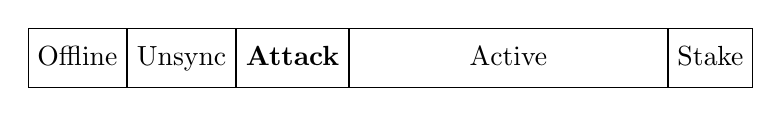
\begin{tikzpicture}[node distance=0.0cm]
    %%%%%%%%%%%%%
    % ACCOUNT A %
    %%%%%%%%%%%%%
    \node (offline) [rec]
        {Offline};
    \node (unsynced) [rec, right = of offline]
        {Unsync};
    \node (attacked) [rec, right = of unsynced]
        {\textbf{Attack}};
    \node (active) [rec, right = of attacked]
        {\quad\quad\quad\quad Active\quad\quad\quad\quad};
    \node (stake) [rec, right = of active]
        {Stake};
    
  \end{tikzpicture}
  \caption{A potential voting arrangement that could lower 51\% attack requirements.}
  \label{fig:attack_dist}
\end{figure}

If an attacker is able to cause Stake \textgreater Active by a combination of these circumstances, they would be able to successfully flip votes on the ledger at the expense of their stake. We can estimate how much this type of attack could cost by examining the market cap of other systems. If we estimate 33\% of representatives are offline or attacked via DoS, an attacker would need to purchase 33\% of the market cap in order to attack the system via voting.

\subsection{Bootstrap Poisoning}
The longer an attacker is able to hold an old private-key with a balance, the higher the probability that balances that existed at that time will not have participating representatives because their balances or representatives have transferred to newer accounts. This means if a node is bootstrapped to an old representation of the network where the attacker has a quorum of voting stake compared to representatives at that point in time, they would be able to oscillate voting decisions to that node. If this new user wanted to interact with anyone besides the attacking node all of their transactions would be denied since they have different head blocks. The net result is nodes can waste the time of new nodes in the network by feeding them bad information. To prevent this, nodes can be paired with an initial database of accounts and known-good block heads; this is a replacement for downloading the database all the way back to the genesis block. The closer the download is to being current, the higher the probability of accurately defending against this attack. In the end, this attack is probably no worse than feeding junk data to nodes while bootstrapping, since they wouldn't be able to transact with anyone who has a contemporary database.

\section{Implementation}
% Status: First Draft; Needs more info from dev team.
Currently the reference implementation is implemented in C++ and has been producing releases since 2014 on Github \cite{LeMahieu_github}.

\subsection{Design Features}
The Nano implementation adheres to the architecture standard outlined in this paper. Additional specifications are described here.

\subsubsection{Signing Algorithm}
Nano uses a modified ED25519 elliptic curve algorithm with Blake2b hashing for all digital signatures \cite{Bernstein_ED25519}. ED25519 was chosen for fast signing, fast verification, and high security.

\subsubsection{Hashing Algorithm}
Since the hashing algorithm is only used to prevent network spam, the algorithm choice is less important when compared to mining-based cryptocurrencies. Our implementation uses Blake2b as a digest algorithm against block contents \cite{Aumasson_blake2}.

\subsubsection{Key Derivation Function}
In the reference wallet, keys are encrypted by a password and the password is fed through a key derivation function to protect against ASIC cracking attempts. Presently Argon2 \cite{Biryukov_argon2} is the winner of the only public competition aimed at creating a resilient key derivation function.

\subsubsection{Block Interval}
Since each account has its own blockchain, updates can be performed asynchronous to the state of network. Therefore there are no block intervals and transactions can be published instantly.

\subsubsection{UDP Message Protocol}
Our system is designed to operate indefinitely using the minimum amount of computing resources as possible. All messages in the system were designed to be stateless and fit within a single UDP packet. This also makes it easier for lite peers with intermittent connectivity to participate in the network without reestablishing short-term TCP connections. TCP is used only for new peers when they want to bootstrap the block chains in a bulk fashion.

Nodes can be sure their transaction was received by the network by observing transaction broadcast traffic from other nodes as it should see several copies echoed back to itself.

\subsection{IPv6 and Multicast}
Building on top of connection-less UDP allows future implementations to use IPv6 multicast as a replacement for traditional transaction flooding and vote broadcast. This will reduce network bandwidth consumption and give more policy flexibility to nodes going forward.

\subsection{Performance}
At the time of this writing, 4.2 million transactions have been processed by the Nano network, yielding a blockchain size of 1.7GB. Transaction times are measured on the order of seconds. A current reference implementation operating on commodity SSDs can process over 10,000 transactions per second being primarily IO bound.

\section{Resource Usage}
This is an overview of resources used by a Nano node. Additionally, we go over ideas for reducing resource usage for specific use cases. Reduced nodes are typically called light, pruned, or simplified payment verification (SPV) nodes.

\subsection{Network}
The network activity of a node is dependent on how much the node contributes towards the health of a network.

\subsubsection{Representative}
A representative node requires maximum network resources as it observes vote traffic from other representatives and publishes its own votes.

\subsubsection{Trustless}
A trustless node is similar to a representative node but is only an observer, it doesn't contain a representative account private key and does not publish votes of its own.

\subsubsection{Trusting}
A trusting node observes vote traffic from one representative it trusts to correctly perform consensus. This cuts down on the amount of inbound vote traffic from representatives going to this node.

\subsubsection{Light}
A light node is also a trusting node that only observes traffic for accounts in which it is interested allowing minimal network usage.

\subsubsection{Bootstrap}
A bootstrap node serves up parts or all of the ledger for nodes that are bringing themselves online. This is done over a TCP connection rather than UDP since it involves a large amount of data that requires advanced flow control.

\subsection{Disk Capacity}
Depending on the user demands, different node configurations require different storage requirements.

\subsubsection{Historical}
A node interested in keeping a full historical record of all transactions will require the maximum amount of storage.

\subsubsection{Current}
Due to the design of keeping accumulated balances with blocks, nodes only need to keep the latest or head blocks for each account in order to participate in consensus. If a node is uninterested in keeping a full history it can opt to keep only the head blocks.

\subsubsection{Light}
A light node keeps no local ledger data and only participates in the network to observe activity on accounts in which it is interested or optionally create new transactions with private keys it holds.

\subsection{CPU}
\subsubsection{Transaction Generating}
A node interested in creating new transactions must produce a Proof of Work nonce in order to pass Nano's throttling mechanism. Computation of various hardware is benchmarked in Appendix \ref{sec:pow_hardware_benchmarks}.

\subsubsection{Representative}
A representative must verify signatures for blocks, votes, and also produce its own signatures to participate in consensus. The amount of CPU resources for a representative node is significantly less than transaction generating and should work with any single CPU in a contemporary computer.

\subsubsection{Observer}
An observer node doesn't generate its own votes. Since signature generation overhead is minimal, the CPU requirements are almost identical to running a representative node.

\section{Conclusion}
In this paper we presented the framework for a trustless, feeless, low-latency cryptocurrency that utilizes a novel block-lattice structure and delegated Proof of Stake voting. The network requires minimal resources, no high-power mining hardware, and can process high transaction throughput. All of this is achieved by having individual blockchains for each account, eliminating access issues and inefficiencies of a global data-structure. We identified possible attack vectors on the system and presented arguments on how Nano is resistant to these forms of attacks.

\appendices
\section{PoW Hardware benchmarks} \label{sec:pow_hardware_benchmarks}
% Status: First Draft; Ready for Review
As mentioned previously, the PoW in RaiBlocks is to reduce network spam.  Our node implementation provides acceleration that can take advantage of OpenCL compatible GPUs. Table~\ref{table:hardware_pow} provides a real-life benchmark comparison of various hardware. Currently the PoW threshold is fixed, but an adaptive threshold may be implemented as average computing power progresses.

\begin{table}[!ht]
\centering
\caption{Hardware PoW Performance}
\label{table:hardware_pow}
\begin{tabular}{ll}
Device                                    & Transactions Per Second \\
\hline
Nvidia Tesla V100 (AWS)                   & 6.4                     \\
Nvidia Tesla P100 (Google,Cloud)          & 4.9                     \\
Nvidia Tesla K80 (Google,Cloud)           & 1.64                    \\
AMD RX 470 OC                             & 1.59                    \\
Nvidia GTX 1060 3GB                       & 1.25                    \\
Intel Core i7 4790K AVX2                  & 0.33                    \\
Intel Core i7 4790K,WebAssembly (Firefox) & 0.14                    \\
Google Cloud 4 vCores                     & 0.14-0.16               \\
ARM64 server 4 cores (Scaleway)           & 0.05-0.07               \\
\end{tabular}
\end{table}
% Appendix one text goes here.

% % you can choose not to have a title for an appendix
% % if you want by leaving the argument blank
% \section{}
% Appendix two text goes here.


% use section* for acknowledgement
\section*{Acknowledgment}
We would like to thank Brian Pugh and B. Cchung for compiling and formatting this paper.

% Can use something like this to put references on a page
% by themselves when using endfloat and the captionsoff option.
\ifCLASSOPTIONcaptionsoff
  \newpage
\fi



% trigger a \newpage just before the given reference
% number - used to balance the columns on the last page
% adjust value as needed - may need to be readjusted if
% the document is modified later
%\IEEEtriggeratref{8}
% The ''triggered'' command can be changed if desired:
%\IEEEtriggercmd{\enlargethispage{-5in}}

% references section

% can use a bibliography generated by BibTeX as a .bbl file
% BibTeX documentation can be easily obtained at:
% http://www.ctan.org/tex-archive/biblio/bibtex/contrib/doc/
% The IEEEtran BibTeX style support page is at:
% http://www.michaelshell.org/tex/ieeetran/bibtex/
%\bibliographystyle{IEEEtran}
% argument is your BibTeX string definitions and bibliography database(s)
%\bibliography{IEEEabrv,../bib/paper}
%
% <OR> manually copy in the resultant .bbl file
% set second argument of \begin to the number of references
% (used to reserve space for the reference number labels box)
%-------------------------------------------------------------------------
{\small
%\bibliographystyle{unsrt}
\bibliographystyle{IEEEtran}
\bibliography{biblio}
}

% biography section
% 
% If you have an EPS/PDF photo (graphicx package needed) extra braces are
% needed around the contents of the optional argument to biography to prevent
% the LaTeX parser from getting confused when it sees the complicated
% \includegraphics command within an optional argument. (You could create
% your own custom macro containing the \includegraphics command to make things
% simpler here.)
%\begin{IEEEbiography}[{\includegraphics[width=1in,height=1.25in,clip,keepaspectratio]{mshell}}]{Michael Shell}
% or if you just want to reserve a space for a photo:

% \begin{IEEEbiography}{Colin LeMahieu}
% Biography text here.
% \end{IEEEbiography}

% if you will not have a photo at all:
% \begin{IEEEbiographynophoto}{John Doe}
% Biography text here.
% \end{IEEEbiographynophoto}

% % insert where needed to balance the two columns on the last page with
% % biographies
% %\newpage

% \begin{IEEEbiographynophoto}{Jane Doe}
% Biography text here.
% \end{IEEEbiographynophoto}

% You can push biographies down or up by placing
% a \vfill before or after them. The appropriate
% use of \vfill depends on what kind of text is
% on the last page and whether or not the columns
% are being equalized.

%\vfill

% Can be used to pull up biographies so that the bottom of the last one
% is flush with the other column.
%\enlargethispage{-5in}



% that's all folks
\end{document}


